% Les tableaux proviennent des CSV du programme.
% Compiler depuis la racine : python3 compiler_rapport.py
\documentclass[a4paper,11pt]{article}
\usepackage[utf8]{inputenc}
\usepackage[T1]{fontenc}
\usepackage[french]{babel}
\usepackage{amsmath,booktabs,graphicx,geometry,listings,float,hyperref}
\geometry{margin=2.1cm}
\graphicspath{{../figures/}}
\hypersetup{hidelinks}
\lstset{basicstyle=\ttfamily\footnotesize,breaklines=true,columns=fullflexible}
\title{TP : comparaison de Sobel, Laplace et Canny}
\author{}\date{20 octobre 2026}
\begin{document}\maketitle

\section{Objectif et protocole}
Ce TP compare les détecteurs de contours Sobel, Laplace et Canny sur un lot de
40 images PGM en niveaux de gris. Chaque image est associée à une référence
\texttt{nom\_gt\_binary.pgm}, dont les contours ont été tracés à la main.
Les références représentent les contours en noir sur fond blanc, tandis que
le programme les produit en blanc sur fond noir.
Le programme est écrit en C++17 et utilise OpenCV 4.11.0.
Les images proviennent de la base de contours de l'université de Groningue :
\url{https://www.cs.rug.nl/~imaging/databases/contour_database/contour_database.html}.
Les annotations manuelles décrivent une sélection de contours et ne reprennent
pas tous les détails visibles dans les images.

La première comparaison utilise un noyau de taille 3 et les seuils suivants :
100 pour Sobel, 30 pour Laplace et 50/150 pour Canny. Les seuils ne sont pas directement comparables entre méthodes,
car les réponses numériques diffèrent. Une seconde expérience les fait varier
sur le même lot afin d'observer le compromis entre les contours conservés
et les réponses parasites. Les réglages sont donc évalués sur ces 40 images,
sans jeu de validation séparé.

\section{Théorie et fonctions OpenCV}
\subsection{Sobel : dérivées premières}
Sobel approxime les dérivées $G_x$ et $G_y$ de l'image par convolution.
Pour un noyau de taille 3,
$K_x=\left(\begin{smallmatrix}-1&0&1\\-2&0&2\\-1&0&1\end{smallmatrix}\right)$,
$K_y=K_x^T$. \texttt{cv::Sobel(image,Gx,CV\_32F,1,0,kernel)} calcule la dérivée
horizontale ; les ordres $(0,1)$ donnent la dérivée verticale.
\texttt{CV\_32F} conserve les valeurs signées sans saturation en 8 bits.
\texttt{cv::magnitude} calcule $M=\sqrt{G_x^2+G_y^2}$, puis
\texttt{cv::compare(M,seuil,edges,CMP\_GE)} garde $M\geq seuil$.
Sans suppression des non-maxima, les contours peuvent être épais.

\subsection{Laplace : dérivée seconde}
Le Laplacien approxime $L=\partial^2I/\partial x^2+\partial^2I/\partial y^2$.
\texttt{cv::Laplacian(image,L,CV\_32F,kernel)} calcule la réponse signée ;
\texttt{cv::absdiff(L,0,A)} donne $|L|$, qui est ensuite seuillé avec
\texttt{cv::compare}. La valeur absolue retient les réponses positives et négatives.
Cette variante ne cherche pas les passages par zéro. Elle peut donner des
réponses épaisses ou doubles et réagit aux variations locales et au bruit.
Un faible seuil retient aussi beaucoup de textures.

\subsection{Canny : amincissement et hystérésis}
Canny estime le gradient et son orientation, supprime les réponses non maximales
et applique une hystérésis. Les réponses dépassant le seuil haut amorcent les
contours ; les plus faibles sont conservées si elles dépassent le seuil bas
et sont reliées à ces contours.
\texttt{cv::Canny(image,edges,bas,haut,kernel)} applique cette procédure.
Le noyau règle l'ouverture du filtre de Sobel : 3, 5 ou 7.
\texttt{L2gradient} reste à \texttt{false}, donc la norme est $|G_x|+|G_y|$,
alors que le calcul de Sobel utilise la norme euclidienne L2.
Un lissage gaussien peut précéder la détection pour réduire l'effet du bruit.
Dans ce programme, l'image est transmise directement à \texttt{cv::Canny},
sans appel préalable à \texttt{cv::GaussianBlur}.
La taille du noyau règle donc le filtre de dérivation, et non l'écart-type
d'un filtre gaussien ajouté à l'image.

Les fonctions Sobel et Laplace acceptent ici les tailles 1, 3, 5 et 7.
La taille du noyau change le voisinage
et l'amplitude des dérivées : le seuil doit être réajusté. Il porte sur des
réponses non normalisées, pas sur les intensités 0--255.
Le seuillage produit un masque binaire 8 bits pour le comptage et la sauvegarde.

\section{Code et utilisation}
\texttt{main.cpp} gère les paramètres, les détecteurs, le calcul des mesures,
le traitement par lot et l'interface.
\texttt{ContourMatching.h} isole l'association des pixels et
\texttt{RadioControls.h} gère les boutons radio de l'interface.
Chaque image est chargée en niveaux de gris, puis traitée par le détecteur choisi.
Les contours obtenus sont comparés à la référence pour calculer les mesures.
Les commandes suivantes permettent de compiler le programme, d'ouvrir
l'interface et de lancer les trois traitements par lot :
\begin{lstlisting}
cmake -S . -B build
cmake --build build -j2
./build/tp_contours --interactive images/bear.pgm
./build/tp_contours --batch images images/gt resultats_sobel sobel 100 150 3
./build/tp_contours --batch images images/gt resultats_laplace laplace 30 150 3
./build/tp_contours --batch images images/gt resultats_canny canny 50 150 3
\end{lstlisting}
Les boutons radio permettent de choisir le détecteur, la taille du noyau
(3, 5 ou 7) et un multiplicateur de seuil (1, 10, 100 ou 1000).
Deux curseurs règlent les seuils. La valeur appliquée est la position du curseur
(de 0 à 2000) multipliée par le facteur choisi. Ce réglage permet d'atteindre
les valeurs élevées nécessaires aux grands noyaux.
Le second seuil est inactif pour Sobel/Laplace. Les seuils Canny de l'interface
sont triés et le bandeau affiche les valeurs réellement appliquées.
La touche Échap, la touche q ou la fermeture de la fenêtre permettent de quitter
l'interface.

Le mode de traitement par lot applique les mêmes paramètres à chaque image.
Il associe chaque image à sa référence et sauvegarde ses contours.
Un fichier CSV regroupe les paramètres, les cinq nombres de pixels et les trois
mesures pour chaque image.

\section{Évaluation avec voisinage 3\texorpdfstring{$\times$}{x}3}
\texttt{threshold} binarise les sorties et inverse les références ;
\texttt{countNonZero} compte les pixels de contour. On note $D$ le nombre de
pixels détectés, $R$ le nombre de pixels de référence et $C$ le nombre de
correspondances retenues. Une correspondance relie deux pixels distants
d'au plus un pixel dans chaque direction, diagonales incluses. Chaque pixel
n'est utilisé qu'une fois. Les cinq grandeurs sont :
\[D,\quad R,\quad C,\quad FP=D-C,\quad FN=R-C.\]
Avec $T=C+FP+FN$, les trois mesures utilisées sont :
\[P=C/T,\qquad TFP=FP/T,\qquad TFN=FN/T.\]
Pour $T>0$, leur somme est 1. Si les deux masques sont vides, les trois ratios
valent 0 par convention, pour éviter une division par zéro.
La performance $P$ mesure la part des correspondances dans cet ensemble.
TFP et TFN mesurent respectivement la part des faux positifs et des faux négatifs,
avec le même dénominateur. Le TFP utilisé ici diffère donc du taux
$FP/(FP+TN)$, qui fait intervenir les vrais négatifs.

\paragraph{Association des pixels.}
Le programme commence par les pixels superposés. Pour chaque détection restante,
il cherche une référence dans son voisinage 3$\times$3. Si cette référence est
déjà prise, il cherche à déplacer la paire existante vers une autre place libre.
Cette recherche maximise le nombre de correspondances, sans réutiliser
un pixel. Un contour épais ne peut donc pas être compté plusieurs fois comme
correct autour d'un seul pixel de référence.

Le voisinage tolère une petite erreur de localisation mais peut la masquer.
L'unicité pénalise les contours épais. Les ratios ne mesurent ni la continuité
ni la pertinence sémantique. Les moyennes suivantes donnent le même poids à
chaque image : ce ne sont pas des ratios de comptes cumulés.

\section{Résultats et interprétation}
\subsection{Réglages principaux}
Les nombres de pixels suivants sont les sommes sur les 40 images : D (détectés),
R (référence), C (corrects), FP (faux positifs), FN (faux négatifs).
\begin{center}\small% Mesures calculées par le programme C++ sur les 40 images.
\begin{tabular}{lrrrrr}
\toprule
Méthode & D & R & C & FP & FN\\
\midrule
Sobel & 1497534 & 229597 & 182421 & 1315113 & 47176\\
Laplace & 4160762 & 229597 & 220467 & 3940295 & 9130\\
Canny & 1499457 & 229597 & 192898 & 1306559 & 36699\\
\bottomrule
\end{tabular}
\end{center}
Les trois ratios ci-dessous sont calculés par image puis moyennés.
\begin{center}% Mesures calculées par le programme C++ sur les 40 images.
\begin{tabular}{lrrr}
\toprule
Méthode & P & TFP & TFN\\
\midrule
Sobel & 0.142958 & 0.806739 & 0.050302\\
Laplace & 0.056167 & 0.940591 & 0.003242\\
Canny & 0.147293 & 0.815878 & 0.036828\\
\bottomrule
\end{tabular}
\end{center}
Canny obtient la performance moyenne la plus élevée (0,147293),
juste devant Sobel (0,142958).
L'écart est faible ; ce classement concerne uniquement les images et les réglages utilisés.
Sobel présente un TFP moyen un peu plus faible que Canny, mais aussi un TFN
moyen plus élevé. Laplace retrouve le plus de pixels de référence :
220\,467 sur 229\,597. Il produit cependant 3\,940\,295 faux positifs,
ce qui explique sa faible performance. Son TFN très bas doit aussi être lu
en tenant compte du dénominateur commun, qui augmente avec les faux positifs.
Les performances restent faibles pour les trois méthodes : une grande partie
des pixels détectés correspond à des détails absents des annotations.

\subsection{Variation des seuils, noyau 3}
\begin{center}% Mesures calculées par le programme C++ sur les 40 images.
\begin{tabular}{lrrrr}
\toprule
Méthode & Seuil(s) & P & TFP & TFN\\
\midrule
Sobel & 50 & 0.069296 & 0.926805 & 0.003900\\
Sobel & 100 & 0.142958 & 0.806739 & 0.050302\\
Sobel & 200 & 0.210627 & 0.430958 & 0.358415\\
Laplace & 15 & 0.037035 & 0.962818 & 0.000146\\
Laplace & 30 & 0.056167 & 0.940591 & 0.003242\\
Laplace & 60 & 0.096405 & 0.865010 & 0.038584\\
Canny & 25/75 & 0.100503 & 0.890334 & 0.009163\\
Canny & 50/150 & 0.147293 & 0.815878 & 0.036828\\
Canny & 100/300 & 0.232391 & 0.545753 & 0.221856\\
\bottomrule
\end{tabular}
\end{center}
Dans les trois séries, augmenter les seuils réduit le TFP et augmente le TFN :
on élimine des réponses parasites mais aussi des contours faibles.
Sobel passe de P=0,069296 à 0,210627 entre 50 et 200, avec un TFN final de 0,358415.
Canny passe de 0,100503 à 0,232391 entre 25/75 et 100/300, avec un TFN de 0,221856.
Parmi ces neuf réglages, Canny 100/300 obtient le meilleur P moyen.
Ce résultat reste propre au lot étudié et ne garantit pas une silhouette
complète sur chaque image.

\clearpage\subsection{Illustrations commentées}
\begin{figure}[H]\centering
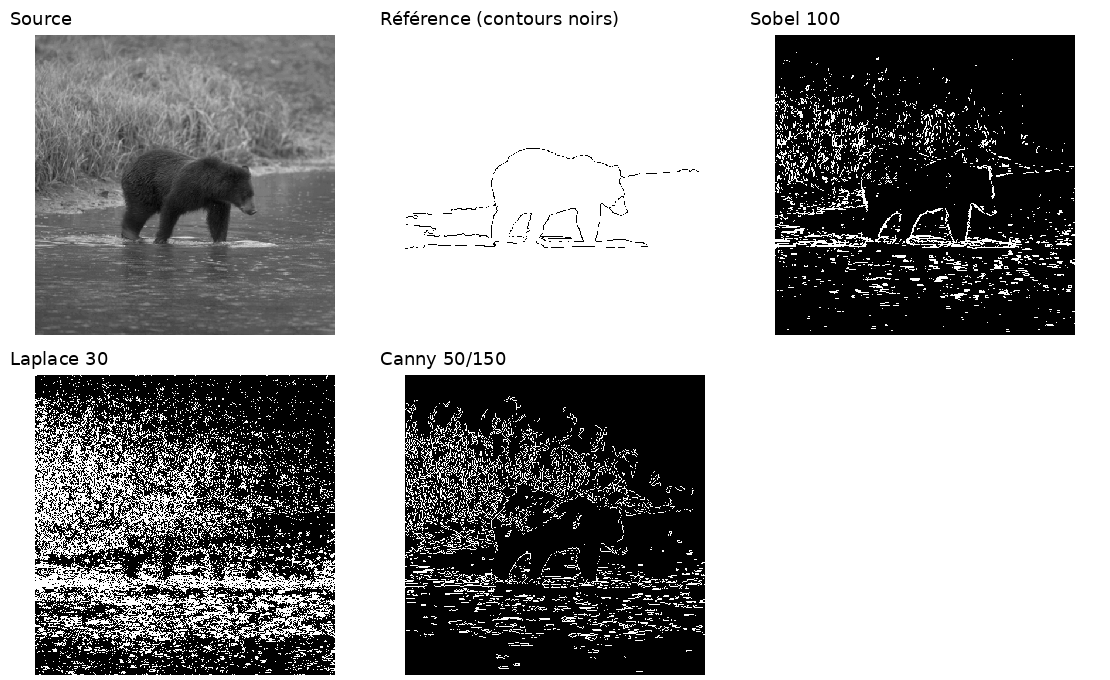
\includegraphics[width=\textwidth]{bear_comparaison.png}
\caption{Ours : source, référence et sorties, noyau 3.}\end{figure}
Dans \texttt{bear}, l'herbe et l'eau produisent beaucoup de contours absents de
la référence. Laplace 30 remplit ces zones ; Sobel 100 conserve aussi des réponses
épaisses. Canny amincit les réponses mais conserve des textures. Un faux positif
selon l'annotation ne signifie pas une absence de contraste réel.
\begin{figure}[H]\centering
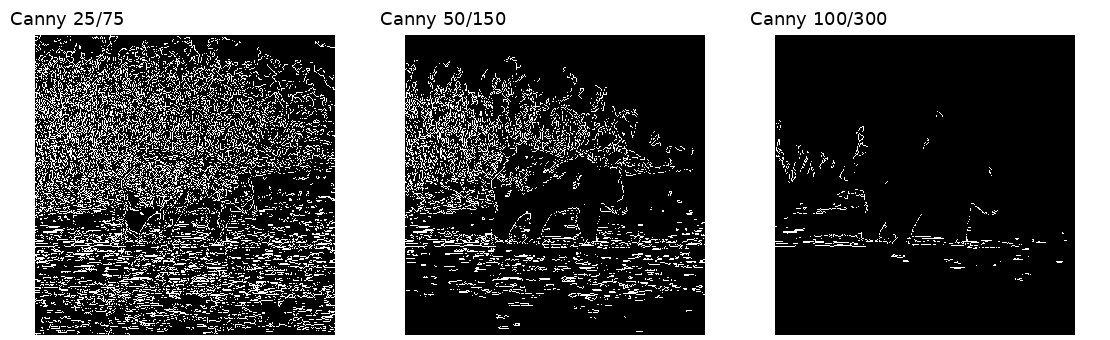
\includegraphics[width=\textwidth]{bear_seuils.png}
\caption{Même ours, trois couples de seuils Canny.}\end{figure}
Avec 100/300, les textures diminuent mais la silhouette de l'ours est fragmentée.
Le réglage qui améliore le score moyen peut donc perdre une partie du contour
de l'objet sur une image particulière.

\clearpage
\begin{figure}[H]\centering
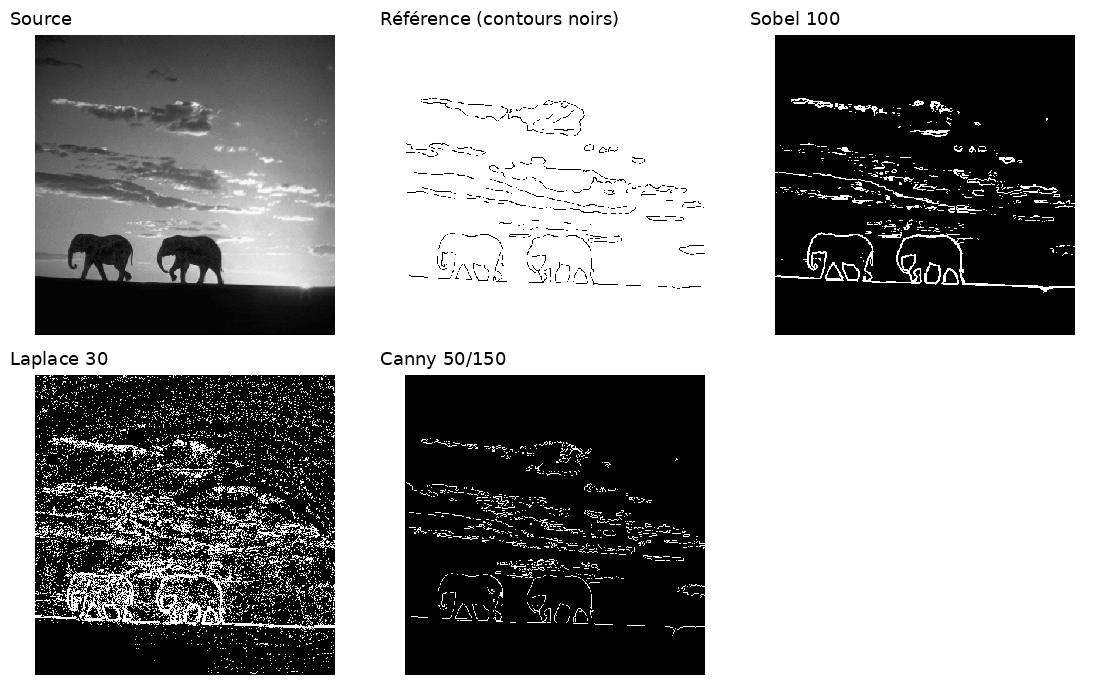
\includegraphics[width=\textwidth]{elephants_comparaison.png}
\caption{Éléphants : silhouettes contrastées et nuages.}\end{figure}
Les silhouettes ressortent bien : Sobel les épaissit, Canny les dessine plus
finement, Laplace ajoute des réponses dans le ciel. Certains nuages figurent
dans la référence et doivent donc être conservés pour cette comparaison.
\begin{figure}[H]\centering
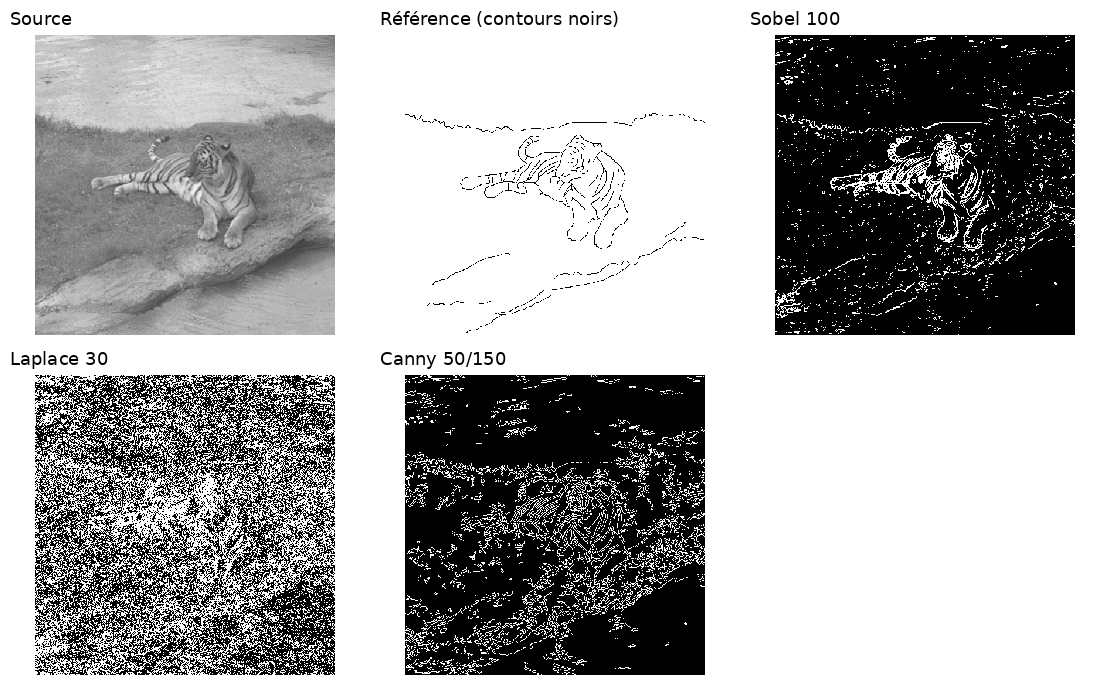
\includegraphics[width=0.85\textwidth]{tiger_comparaison.png}
\caption{Tigre : pelage, sol et tronc.}\end{figure}
Le pelage produit des détails seulement partiellement annotés ; les textures du
sol et du tronc augmentent les faux positifs. Cet exemple montre l'intérêt d'examiner la
localisation des réponses et les détails conservés en complément des mesures.

\section{Bilan de la comparaison}
Avec les réglages principaux, Canny obtient la meilleure performance moyenne,
juste devant Sobel. Laplace retrouve davantage de pixels de référence mais
ajoute beaucoup de faux positifs. Augmenter les seuils retire des textures,
mais fait aussi disparaître des contours utiles.

Le voisinage 3$\times$3 accepte un petit décalage : c'est utile pour comparer
les détecteurs à un tracé manuel, mais cela rend les mesures moins sensibles
aux erreurs de localisation. L'association unique évite de favoriser les
contours épais. En revanche, les mesures n'indiquent pas si une silhouette
est continue. Les références ne contiennent pas tous les détails visibles.
Le choix des paramètres repose donc sur les mesures et sur les images.

\end{document}
